\begin{figure}[!ht]
\centering
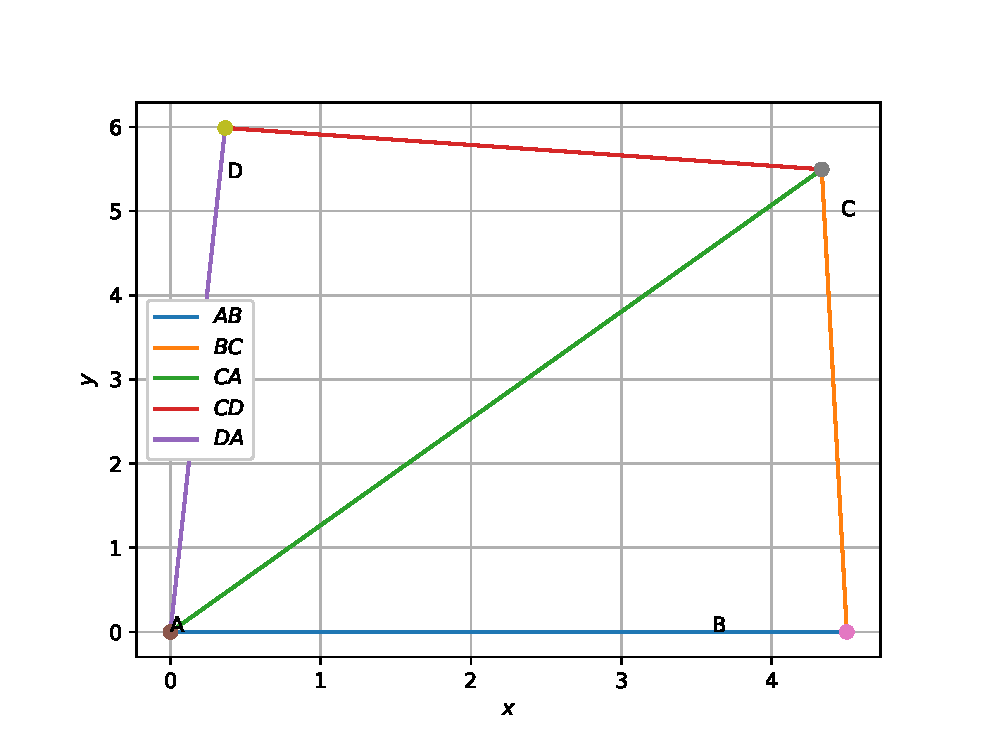
\includegraphics[width= \columnwidth]{./solutions/7/figs/quad/quad.eps}
\caption{Square ABCD}
\label{fig:2.2.7}
\end{figure}
See Fig. \ref{fig:2.2.7}.

\begin{enumerate}
\item From inspection we see that the opposite vertices forms a diagonal which is parallel to x-axis. Then the diagonal formed by other two vertices is parallel to y-axis(i.e. their x coordinates are equal). Let $\vec{A}= \myvec{-1\\2}$  and $\vec{C}=\myvec{3\\2}$. 

\item Diagonals bisect each other at 90\degree.
Let $\vec{B}$ and $\vec{D}$ be other two vertices. 
\item Using the property that diagonals bisect each other at 90\degree, we can obtain other vertices by rotating diagonal AC by 90\degree about $\vec{E}$ in clockwise or anticlockwise direction.

\item The rotation matrix for a rotation of angle 90\degree about origin in anticlockwise direction is given by
\begin{align}
\myvec{\cos90\degree&-\sin90\degree\\\sin90\degree&\cos90\degree}=\myvec{0&-1\\1&0}
\end{align}
The $\vec{E}$ is given by
\begin{align}
\vec{E}&= \frac{\vec{A}+\vec{C}}{2} \\
&= \myvec{1\\2}
\end{align}

\item To make the rotation we need to shift the $\vec{E}$ to origin. So the change in other vectors are
\begin{align}
\vec{A}-\vec{E}&=\myvec{-2\\0}\\
\vec{C}-\vec{E}&=\myvec{2\\0}
\end{align}

The required matrix now is $\myvec{-2&2\\0&0}$. Multiplying this with rotation matrix 
\begin{align}
&= \myvec{0&-1\\1&0}\myvec{-2&2\\0&0}\\
&=\myvec{0&0\\-2&2}
\end{align}
Now we obtained the coordinates as $\myvec{0\\-2}$ and $\myvec{0\\2}$.
To obtain the final coordinates we will add $\vec{E}$ to shift to the actual position.
\begin{align}
\vec{B}=\myvec{0\\-2}+\myvec{1\\2}\\
\vec{D}=\myvec{0\\2}+\myvec{1\\2}
\end{align}
Thus 
\begin{align}
\vec{B}&= \myvec{1\\0} \\
\vec{D}&= \myvec{1\\4}
\end{align} 
\item The python code for the figure can be downloaded from
\begin{lstlisting}
solutions/7/codes/quad/quad.py
\end{lstlisting}
\end{enumerate}  
